% Options for packages loaded elsewhere
\PassOptionsToPackage{unicode}{hyperref}
\PassOptionsToPackage{hyphens}{url}
\PassOptionsToPackage{dvipsnames,svgnames,x11names}{xcolor}
%
\documentclass[
  letterpaper,
  DIV=11,
  numbers=noendperiod]{scrartcl}

\usepackage{amsmath,amssymb}
\usepackage{iftex}
\ifPDFTeX
  \usepackage[T1]{fontenc}
  \usepackage[utf8]{inputenc}
  \usepackage{textcomp} % provide euro and other symbols
\else % if luatex or xetex
  \usepackage{unicode-math}
  \defaultfontfeatures{Scale=MatchLowercase}
  \defaultfontfeatures[\rmfamily]{Ligatures=TeX,Scale=1}
\fi
\usepackage{lmodern}
\ifPDFTeX\else  
    % xetex/luatex font selection
\fi
% Use upquote if available, for straight quotes in verbatim environments
\IfFileExists{upquote.sty}{\usepackage{upquote}}{}
\IfFileExists{microtype.sty}{% use microtype if available
  \usepackage[]{microtype}
  \UseMicrotypeSet[protrusion]{basicmath} % disable protrusion for tt fonts
}{}
\makeatletter
\@ifundefined{KOMAClassName}{% if non-KOMA class
  \IfFileExists{parskip.sty}{%
    \usepackage{parskip}
  }{% else
    \setlength{\parindent}{0pt}
    \setlength{\parskip}{6pt plus 2pt minus 1pt}}
}{% if KOMA class
  \KOMAoptions{parskip=half}}
\makeatother
\usepackage{xcolor}
\setlength{\emergencystretch}{3em} % prevent overfull lines
\setcounter{secnumdepth}{-\maxdimen} % remove section numbering
% Make \paragraph and \subparagraph free-standing
\makeatletter
\ifx\paragraph\undefined\else
  \let\oldparagraph\paragraph
  \renewcommand{\paragraph}{
    \@ifstar
      \xxxParagraphStar
      \xxxParagraphNoStar
  }
  \newcommand{\xxxParagraphStar}[1]{\oldparagraph*{#1}\mbox{}}
  \newcommand{\xxxParagraphNoStar}[1]{\oldparagraph{#1}\mbox{}}
\fi
\ifx\subparagraph\undefined\else
  \let\oldsubparagraph\subparagraph
  \renewcommand{\subparagraph}{
    \@ifstar
      \xxxSubParagraphStar
      \xxxSubParagraphNoStar
  }
  \newcommand{\xxxSubParagraphStar}[1]{\oldsubparagraph*{#1}\mbox{}}
  \newcommand{\xxxSubParagraphNoStar}[1]{\oldsubparagraph{#1}\mbox{}}
\fi
\makeatother


\providecommand{\tightlist}{%
  \setlength{\itemsep}{0pt}\setlength{\parskip}{0pt}}\usepackage{longtable,booktabs,array}
\usepackage{calc} % for calculating minipage widths
% Correct order of tables after \paragraph or \subparagraph
\usepackage{etoolbox}
\makeatletter
\patchcmd\longtable{\par}{\if@noskipsec\mbox{}\fi\par}{}{}
\makeatother
% Allow footnotes in longtable head/foot
\IfFileExists{footnotehyper.sty}{\usepackage{footnotehyper}}{\usepackage{footnote}}
\makesavenoteenv{longtable}
\usepackage{graphicx}
\makeatletter
\newsavebox\pandoc@box
\newcommand*\pandocbounded[1]{% scales image to fit in text height/width
  \sbox\pandoc@box{#1}%
  \Gscale@div\@tempa{\textheight}{\dimexpr\ht\pandoc@box+\dp\pandoc@box\relax}%
  \Gscale@div\@tempb{\linewidth}{\wd\pandoc@box}%
  \ifdim\@tempb\p@<\@tempa\p@\let\@tempa\@tempb\fi% select the smaller of both
  \ifdim\@tempa\p@<\p@\scalebox{\@tempa}{\usebox\pandoc@box}%
  \else\usebox{\pandoc@box}%
  \fi%
}
% Set default figure placement to htbp
\def\fps@figure{htbp}
\makeatother

\KOMAoption{captions}{tableheading}
\makeatletter
\@ifpackageloaded{caption}{}{\usepackage{caption}}
\AtBeginDocument{%
\ifdefined\contentsname
  \renewcommand*\contentsname{Table of contents}
\else
  \newcommand\contentsname{Table of contents}
\fi
\ifdefined\listfigurename
  \renewcommand*\listfigurename{List of Figures}
\else
  \newcommand\listfigurename{List of Figures}
\fi
\ifdefined\listtablename
  \renewcommand*\listtablename{List of Tables}
\else
  \newcommand\listtablename{List of Tables}
\fi
\ifdefined\figurename
  \renewcommand*\figurename{Figure}
\else
  \newcommand\figurename{Figure}
\fi
\ifdefined\tablename
  \renewcommand*\tablename{Table}
\else
  \newcommand\tablename{Table}
\fi
}
\@ifpackageloaded{float}{}{\usepackage{float}}
\floatstyle{ruled}
\@ifundefined{c@chapter}{\newfloat{codelisting}{h}{lop}}{\newfloat{codelisting}{h}{lop}[chapter]}
\floatname{codelisting}{Listing}
\newcommand*\listoflistings{\listof{codelisting}{List of Listings}}
\makeatother
\makeatletter
\makeatother
\makeatletter
\@ifpackageloaded{caption}{}{\usepackage{caption}}
\@ifpackageloaded{subcaption}{}{\usepackage{subcaption}}
\makeatother

\usepackage{bookmark}

\IfFileExists{xurl.sty}{\usepackage{xurl}}{} % add URL line breaks if available
\urlstyle{same} % disable monospaced font for URLs
\hypersetup{
  pdftitle={Assignment 1 - Report},
  colorlinks=true,
  linkcolor={blue},
  filecolor={Maroon},
  citecolor={Blue},
  urlcolor={Blue},
  pdfcreator={LaTeX via pandoc}}


\title{Assignment 1 - Report}
\author{}
\date{}

\begin{document}
\maketitle


\subsection{Abstract}\label{abstract}

Forecast avalanche hazard (FAH) is reported on an ordered five-level
scale, making the correct ordering of predictions as important as the
exact class assignment. We build a modelling-ready dataset from
operational observations in Scotland and cast next-day FAH as an ordinal
forecasting problem. Data preparation standardises identifiers, audits
and repairs missingness, applies physically sensible bounds, encodes
circular variables with sine--cosine pairs, and adds seasonal
day-of-year features. We split chronologically (80/20) with an embargo
to avoid look-ahead.

For modelling, we turn each area's history into 14-day windows of
dynamic features, fuse static site attributes, and train an LSTM with a
CORN ordinal head that predicts \(K - 1\) exceedance probabilities.
Class imbalance is handled by oversampling rare classes in minibatches
and class-balanced per-threshold weights in the loss. We then tune
monotone thresholds on the most recent validation fold to convert
probabilities into labels.

Validation uses forward-chaining time folds; evaluation on a held-out
test window reports Accuracy, Macro-F1, MAE, and Quadratic Weighted
Kappa (QWK). Compared with three simple baselines (global majority,
per-area majority, and persistence), the LSTM--CORN model improves
ordinal-aware agreement (QWK) and reduces absolute error (MAE), with
most mistakes within one level of the truth. Limitations include
scarcity of High hazard days and potential sensitivity to the temporal
split, but the approach is reproducible and operationally realistic, and
it provides a clear path to calibration and extension.

\subsection{Introduction}\label{introduction}

Avalanche hazard is reported on an ordered five-level scale, making the
correct ordering of predictions as important as the exact class
assignment. According to the Conceptual Model of Avalanche Hazard
(Statham et al., 2018), the hazard level is determined by combining two
ordinal variables---likelihood of avalanche occurrence and destructive
size---into a single danger rating. This motivates treating FAH as an
ordinal rather than a nominal target.

This project assembles a modelling-ready dataset from Scottish
observations and frames next-day Forecast Avalanche Hazard (FAH) as an
ordinal forecasting problem. Data preparation (in R) standardises
identifiers, audits and repairs missing values, applies physical
plausibility checks, encodes circular angles as sine/cosine, and adds
day-of-year seasonality. Model matrices are exported with an ordered
target, and a chronological \(80/20\) split prevents look-ahead.

Methodologically, we use a sequence model to reflect that hazard depends
on recent conditions. We frame each area--day as a one-step-ahead
forecast and feed the model a fixed 14-day look-back of daily predictors
together with static site attributes. This mirrors the standard
time-series set-up in which inputs comprise a recent window of
observations plus static metadata (Lim and Zohren, 2021; Eq. 2.1). We
implement the encoder with an LSTM over the 14-day window and
concatenate the static features before the output layer.

For the ordinal output layer we adopt CORN (Conditional Ordinal
Regression for Neural Networks). CORN decomposes a \(K\)-class ordered
target into \(K - 1\) conditional exceedance tasks that estimate
\(P(y > k \mid y > k - 1)\); the unconditional exceedance probabilities
\(P(y > k)\) follow by the probability chain rule, which guarantees
rank-consistent (non-increasing) probabilities across thresholds. Final
class labels are obtained by thresholding these \(K - 1\) probabilities
and counting exceedances (Cao, Mirjalili and Raschka, 2020).

Because High levels are rare, we address class imbalance in two ways.
First, we oversample minority classes within batches. Second, we apply
the class-balanced loss based on the effective number of samples, which
weights each class by \((1 - \beta)/(1 - \beta^{n_c})\) so rare classes
have more influence without fabricating data (Cui et al., 2019, Sec. 3).

Validation uses forward-chaining folds with a 10-day embargo to reflect
operational constraints. Model performance is evaluated on a held-out
test window using Accuracy, Macro-F1, MAE, and Quadratic Weighted Kappa
(QWK). Three baseline models are used for comparison: global majority,
per-area majority, and persistence (yesterday's value). All code is
reproducible, with deterministic seeds and cached lookups, and all
preprocessing parameters are fit on the training data and then applied
to the test set through a baked pipeline.

\subsection{Data \& Methods}\label{data-methods}

\subsubsection{Data}\label{data}

We analysed a 2009--2025 archive of daily avalanche forecasts from the
Scottish Avalanche Information Service across six forecasting regions.
The prediction target is the forecast avalanche hazard (FAH) for the
following day, encoded as an \emph{ordered} categorical variable with
levels:

\emph{Low \textless{} Moderate \textless{} Considerable -- \textless{}
Considerable + \textless{} High}

Predictors comprise:\\
1. \textbf{Site and topography} --- OS grid identifier, location name,
longitude, latitude, altitude, incline.\\
2. \textbf{Contemporaneous meteorology} near the forecast location ---
summit air temperature, summit wind speed and direction, lower-level
winds, cloud, and insolation.\\
3. \textbf{Snowpack observations} derived from field tests --- snow
temperature, maximum temperature and hardness gradients, foot and ski
penetration indices, crystal type, wetness, and a derived stability
index.

To avoid information leakage for the FAH task, the observed hazard on
the following day (OAH) was removed from the analysis dataset.

\subsubsection{Methods: Data Preparation, Cleaning, and
Pre-processing}\label{methods-data-preparation-cleaning-and-pre-processing}

\paragraph{1. Type standardisation and initial feature
engineering}\label{type-standardisation-and-initial-feature-engineering}

We converted timestamps to Date and derived year, month, day-of-year
(\texttt{doy}), and meteorological season (DJF/MAM/JJA/SON). Identifiers
and descriptors were given sensible types (e.g., \texttt{Area} as a
factor; OS grid and location as character). The hazard response was
stored as an ordered factor (\texttt{FAH\_ord}) using the level order
defined above. These steps preserve the outcome's ordinal structure for
modelling and evaluation and add explicit seasonality features for
downstream encoding.

\paragraph{2. Spatial consistency
checks}\label{spatial-consistency-checks}

We examined whether OS grids denote unique points. Longitude and
latitude vary within OS grids, indicating that an OS grid represents an
area rather than a single coordinate. Altitude is not constant within OS
grids. Accordingly, altitude should not be imputed from the OS grid
identifier alone: since each grid covers heterogeneous terrain, we
instead query elevation using the precise latitude-longitude
coordinates.

\paragraph{3. Record keys, duplicates, and
consolidation}\label{record-keys-duplicates-and-consolidation}

We treated (Date, OSgrid, Area) as the record key. For any key with
multiple rows, we counted---column by column---how many distinct
non-missing values appeared.

\begin{itemize}
\tightlist
\item
  If the duplicates differed only by missing values, we collapsed them
  to a single row, taking the first available non-missing value in each
  column.\\
\item
  If any column showed truly conflicting observations (more than one
  distinct non-missing value), we kept all rows for that key and flagged
  the group as conflicted.
\end{itemize}

This approach preserves genuine differences, avoids inventing data, and
leaves a clear audit trail wherever sources disagree.

\paragraph{4. Missingness audit and design of
indicators}\label{missingness-audit-and-design-of-indicators}

We first measured missingness per variable and inspected its pattern.
Where the absence itself could be informative, we created explicit 0/1
``was-missing'' flags (before any outlier recoding). These indicators
were made for: AV.cat, Ski.pen, Crystals, Wetness, Snow.Index, and the
summit weather fields (Summit.Wind.Dir, Summit.Wind.Speed,
Summit.Air.Temp). Doing this early ensures the indicators reflect the
data as collected and aren't confounded by later plausibility filters.

Some fields (e.g., Max.Temp.Grad, Max.Hardness.Grad) are only measured
when a snow pit is carried out. When no pit is done those fields are
blank by design, so we did not add extra ``missing'' indicators;
instead, we impute those numeric blanks downstream for modelling.

\textbf{Snow.Index check:} Because many values are exactly zero, we
tested whether Snow.Index == 0 was being used as a stand-in for ``no
test.'' It wasn't: rows with Snow.Index = 0 didn't show elevated
missingness in pit variables, so zeros appear to be legitimate
measurements (e.g., stable conditions). We therefore kept zeros as valid
values and treated only NA as missing.

\paragraph{5. Physically defensible plausibility
filters}\label{physically-defensible-plausibility-filters}

We applied conservative real-world plausibility checks and recoded any
violations to \texttt{NA} so they can be handled by imputation rather
than ad-hoc edits. The limits reflect basic constraints (e.g., angles in
\(0{-}360^\circ\), non-negative depths) and local context.

\begin{itemize}
\tightlist
\item
  Directional variables (Aspect, Wind.Dir, Summit.Wind.Dir): values
  outside \([0^\circ, 360^\circ]\) set to \texttt{NA}.\\
\item
  Snow temperature (\(^\circ\)C): values \(> 5\) set to NA (snow cannot
  persist above \(\sim 0^\circ\)C; a small buffer accommodates sensor
  and entry noise).\\
\item
  Insolation (index): values outside \(0{-}20\) set to NA.\\
\item
  Incline (\(^\circ\)): values \(<0\) or \(>90\) set to NA.\\
\item
  Foot penetration (cm): values \(<0\) or \(>100\) set to NA.\\
\item
  Total snow depth (cm): values \(<0\) or \(>500\) set to NA (regional
  plausibility).\\
\item
  Maximum temperature gradient (\(^\circ\)C/10 cm): values \(> 10\) set
  to NA.\\
\item
  Altitude (m): values \(<0\) or \(>1400\) set to NA (Scotland's highest
  peak \(\approx 1345\) m).
\end{itemize}

Marking impossible readings as \texttt{NA} prevents them from skewing
summaries or model fits and lets the downstream multivariate imputer
estimate plausible replacements from the remaining data.

\paragraph{6. Altitude repair via coordinate-based elevation
lookup}\label{altitude-repair-via-coordinate-based-elevation-lookup}

For the small number of missing altitudes, we queried an open elevation
service at rounded (\texttt{latitude}, \texttt{longitude}) and filled
\texttt{Alt} where a value was returned. One queried coordinate yielded
\(0\) m (a sea-loch), indicating a geolocation error. For that single
case, we replaced the coordinate with the area mean (Creag Meagaidh) and
re-queried. To ensure deterministic compilation, elevation results are
cached locally; subsequent runs read from cache if the service is
unavailable.

\paragraph{7. Circular encodings for directional
variables}\label{circular-encodings-for-directional-variables}

\textbf{Circular encodings for directional variables.} Because angles
wrap around at \(360^\circ\), treating them as ordinary numbers creates
an artificial jump between \(359^\circ\) and \(0^\circ\). We therefore
replaced each directional variable (\texttt{Wind.Dir},
\texttt{Summit.Wind.Dir}, \texttt{Aspect}) with two new variables that
locate the direction on the unit circle: the sine and cosine of the
angle (in radians). This keeps \(0^\circ\) and \(360^\circ\) close in
feature space, and removes the wrap-around discontinuity, which helps
and yields smoother relationships for the models. Missing angles
remained missing in both components and were imputed later.

\paragraph{8. Time-aware splitting and leakage
control}\label{time-aware-splitting-and-leakage-control}

The data was split chronologically into \(80\%\) training and \(20\%\)
test by calendar time (no overlap).Any rows missing a \texttt{Date} or
the target (\texttt{FAH\_ord}) were dropped before the split. We checked
class balance in each split; the High level is very rare and does not
appear in the test window (so performance on that class cannot be
evaluated). All preprocessing steps were fit on the training set only
(e.g., imputation, scaling, encoding) and then applied unchanged to the
test set. This setup avoids information leakage.

\paragraph{9. Pre-processing pipeline for modelling
(recipes)}\label{pre-processing-pipeline-for-modelling-recipes}

A single, train-fitted \texttt{recipes} pipeline was implemented with
the following stages:

\begin{enumerate}
\def\labelenumi{\arabic{enumi}.}
\tightlist
\item
  \textbf{Column exclusion:} Dropped identifiers and free text, raw time
  stamps, and raw angles: \texttt{OSgrid}, \texttt{Location},
  \texttt{Date}, \texttt{DateTime}, raw \texttt{Wind.Dir}, raw
  \texttt{Summit.Wind.Dir}, and raw \texttt{Aspect}. The raw target FAH
  was excluded in favour of \texttt{FAH\_ord}.\\
\item
  \textbf{Rare-level consolidation:} Collapsed very rare categorical
  levels to \texttt{"other"} using \(\texttt{threshold} = 0.005\) to
  avoid sparse dummies.\\
\item
  \textbf{Imputation:} Categorical variables were imputed by mode;
  numerical variables by bagged-tree imputation (bootstrap ensembles
  estimated on the training data), which captures non-linearities and
  interactions in mixed meteorological and snowpack features more
  effectively than mean or KNN imputation.\\
\item
  \textbf{Encoding:} One-hot encoding of categorical predictors
  (including \texttt{Area}).\\
\item
  \textbf{Variance filtering:} Removal of zero-variance and
  near-zero-variance predictors.\\
\item
  \textbf{Scaling:} Standardisation of numerical predictors, excluding
  the 0/1 informative-missing indicators (and area dummies) to preserve
  their interpretability.\\
\item
  \textbf{Seasonality:} Replacement of discrete season dummies with
  smooth cyclical features \(doy\_sin\) and \(doy\_cos\) (constructed
  from day-of-year with leap years handled); season binaries were
  removed to reduce collinearity.\\
\item
  \textbf{Target mapping:} The ordered response was mapped once to
  integers \(0{-}4\) to provide a single source of truth for
  neural-network models.
\end{enumerate}

The recipe was prepped on the training set (estimating imputation
models, encoding maps, and scaling parameters) and then baked on both
training and test splits to yield model-ready matrices
(\texttt{x\_train}, \texttt{x\_test}). For downstream modelling and
plotting, a \texttt{Date} column was retained; final matrices
(\(X\_{train}\), \(X\_{test}\)) include the integer-encoded target as
the last column.

\paragraph{10. Reproducibility, diagnostics, and
assumptions}\label{reproducibility-diagnostics-and-assumptions}

We fixed random seeds and kept all data-prep and modelling steps in a
single scripted pipeline so that results are reproducible across runs.
After baking the recipe, there were no remaining missing values in
either split. We re-checked the composite key (\texttt{Date},
\texttt{OSgrid}, \texttt{Area}) after duplicate handling, and we
spot-checked distributions of imputed variables to make sure they looked
reasonable (plots not shown for space). Elevation queries are cached
locally, so reruns do not depend on the external service.

Our working assumptions were:\\
(i) the value ranges we used to flag implausible measurements reflect
Scottish conditions;\\
(ii) \texttt{Snow.Index\ ==\ 0} is a \textbf{valid zero} (stable
conditions), not a stand-in for ``no test''; and\\
(iii) the ``informative-missing'' indicators genuinely capture absence
at the time of collection rather than artefacts created later in
cleaning.

\paragraph{11. Limitations and sensitivity
considerations}\label{limitations-and-sensitivity-considerations}

The High hazard class is rare (and absent in our test window) so
standard accuracy alone can be misleading. We therefore report
macro-averaged scores and discuss calibration in the results, but
performance on the very rarest conditions remains uncertain. The
plausibility cut-offs (e.g., the threshold for snow temperature) are
conservative choices, not unique truths; reasonable alternatives could
be used, and results may shift slightly.\\
Finally, because we split by time, outcomes can vary with the split date
(e.g., if conditions change from one season to the next). This is
typical in operational forecasting; sensitivity checks (e.g., alternate
split points or small variations in thresholds and look-back length)
would be a natural extension.

\subsubsection{Methods: Neural ordinal forecasting
model}\label{methods-neural-ordinal-forecasting-model}

This stage uses Python (PyTorch) to learn an ordinal mapping from the
feature set prepared in R to the next-day hazard level (FAH). We (i)
convert the tabular data into area-wise sequences with a 14-day
look-back, (ii) train an LSTM + CORN head (Cumulative Ordinal Regression
for Neural networks), (iii) handle imbalance by oversampling and
class-balanced per-threshold weights, and (iv) tune monotone decision
thresholds for converting CORN probabilities to class labels.

OR:

We model next-day FAH (levels \(0\)--\(4\)) as an ordinal problem in
PyTorch (Python). From the R-prepared matrices we build area-wise 14-day
look-back sequences and train an LSTM with a CORN head (Cumulative
Ordinal Regression for Neural Networks). We address class imbalance via
oversampling and class-balanced per-threshold weights, then tune
monotone (non-increasing) thresholds to turn CORN probabilities into
class labels. Validation is time-aware (forward-chaining folds with a
10-day embargo), and early stopping uses Quadratic Weighted Kappa (QWK).

\begin{verbatim}
<torch._C.Generator object at 0x00000286E94662F0>
\end{verbatim}

\paragraph{1. Data interface and temporal
windows}\label{data-interface-and-temporal-windows}

We read the preprocessed matrices exported from R
(\texttt{X\_train.csv}, \texttt{X\_test.csv}). The response is the
ordered integer
\texttt{FAH\_ord\ \textbackslash{}in\ \textbackslash{}\{0,\ \textbackslash{}ldots,\ 4\textbackslash{}\}}
and a \texttt{Date} column is retained for temporal alignment.

For sequential learning we constructed area-wise sliding windows with
look-back \(L = 14\) days and horizon \(H = 0\) (predict today's FAH
from the previous 14 days) (Lim and Zohren, 2021; Eq. 2.1). Predictors
were split into:

\begin{itemize}
\tightlist
\item
  \textbf{Static features} (fed once per window): longitude, latitude,
  altitude, incline, and the one-hot area indicators.\\
\item
  \textbf{Dynamic features} (fed as a length-\(L\) (\(14\)) sequence):
  all remaining numeric predictors after excluding static variables and
  the target. We also engineered \texttt{FAH\_prev} (yesterday's (FAH)
  hazard within the same area) and included it among the dynamic
  features. It is available operationally and does not leak future
  labels.\\
\end{itemize}

The train/test boundary follows the R split (\(80\%\) earliest dates for
training; remaining \(20\%\) for testing). Windows are built after
concatenating and then filtering by the \textbf{target date} so that
nothing from the test period influences training.

\paragraph{2. Architecture and loss
(CORN--LSTM)}\label{architecture-and-loss-cornlstm}

The network is an \textbf{LSTM} over the dynamic sequence. We take its
last hidden state, concatenate it with the static features, pass it
through a small MLP head, and then through a CORN layer.

\begin{itemize}
\tightlist
\item
  \textbf{CORN (Formulation and Rationale):} Instead of a single
  \(K\)-way softmax, CORN produces \(K - 1\) logits that answer ordered
  questions \(\Pr(y > 0)\), \(\Pr(y > 1)\), \(\ldots\),
  \(\Pr(y > K - 2)\). Because these events become harder as \(k\) grows,
  their probabilities naturally decrease with \(k\) (Cao, Mirjalili and
  Raschka, 2020).
\item
  \textbf{Training:} We compute CORN targets from the true class and
  minimise binary cross-entropy on the \(K - 1\) logits.
\item
  \textbf{Prediction:} At inference, we threshold the \(K - 1\)
  probabilities, count how many exceed their thresholds, and that count
  is the predicted FAH level.
\item
  \textbf{Validation metric:} We report \textbf{Quadratic Weighted Kappa
  (QWK)}, which rewards getting close on an ordinal scale (e.g., a
  \(2 \leftrightarrow 3\) mistake is penalised less than
  \(0 \leftrightarrow 4\)).
\end{itemize}

\paragraph{3. Class imbalance handling}\label{class-imbalance-handling}

High hazard levels are rare. We address this imbalance in two ways:

\begin{enumerate}
\def\labelenumi{\arabic{enumi}.}
\tightlist
\item
  \textbf{Batch oversampling:} Oversampling in the training loader
  (\texttt{WeightedRandomSampler}) to increase the frequency of rarer
  FAH levels during optimisation, so minority levels appear more often
  in batches.\\
\item
  \textbf{Class-balanced CORN loss:} For each threshold \(k\), we
  compute a positive weight using the ``effective number of samples''
  (\(\beta = 0.999\)) and apply it in the BCE term, so rare exceedance
  events \((y > k)\) contribute proportionally more without duplicating
  data (Cui et al., 2019).
\end{enumerate}

\paragraph{4. Validation protocol, hyperparameter search, and early
stopping}\label{validation-protocol-hyperparameter-search-and-early-stopping}

We created \textbf{forward-chaining time folds} (\(K=5\)) with a
\textbf{10-day embargo} before each validation slice to avoid look-ahead
leakage. We tuned hyperparameters with \textbf{Optuna} over:

\begin{itemize}
\tightlist
\item
  hidden size \(\{32, 48, 64\}\),\\
\item
  number of LSTM layers \(\{1, 2\}\),\\
\item
  head dropout \([0.1, 0.5]\),\\
\item
  RNN dropout (only if \(\geq 2\) layers),~
\item
  learning rate \([10^{-4}, 3 \times 10^{-3}]\),\\
\item
  weight decay \([10^{-6}, 10^{-3}]\),\\
\item
  batch size \(\{128, 256, 512\}\).
\end{itemize}

The objective was to maximise the mean QWK across folds. Training used
Adam, gradient-norm clipping (1.0), and early stopping on validation
QWK. After selection, the model was refit on all training windows and
thresholds were calibrated on the most recent validation fold, then
fixed for test.

\paragraph{\texorpdfstring{5. Threshold calibration (monotone
\(\tau\))}{5. Threshold calibration (monotone \textbackslash tau)}}\label{threshold-calibration-monotone-tau}

CORN outputs \(K - 1\) probabilities. To turn them into labels, we tune
monotone thresholds \(\tau_1 \ge \tau_2 \ge \cdots \ge \tau_{K-1}\) on
the latest validation fold using a simple grid over \(0.3\)--\(0.7\),
selecting the vector that maximises QWK. The monotonicity is
non-increasing because \(\Pr(y > k)\) decreases with \(k\); later
thresholds should never be easier to exceed than earlier ones.

The tuned vector used for test was:

\[
\tau = [0.52, \; 0.50, \; 0.50, \; 0.48].
\]

\paragraph{6. Final refit and test
evaluation}\label{final-refit-and-test-evaluation}

We refit the model on all training windows, keeping a small,
chronological \(90/10\) tail for early stopping. We then evaluate once
on the held-out test windows using the fixed \(\tau\) vector above.
Metrics reported are Accuracy, Macro-F1, MAE, and QWK, and include a
confusion matrix and a per-class report in the Results.

\begin{verbatim}
488
\end{verbatim}

\paragraph{7. Baselines}\label{baselines}

For context, we implemented three simple non-parametric reference models
as baselines (all fitted only on training labels).

\begin{enumerate}
\def\labelenumi{(\roman{enumi})}
\tightlist
\item
  a \textbf{global majority} classifier that predicts the most frequent
  FAH level in the training labels,\\
\item
  a \textbf{per-area majority} classifier that uses the most frequent
  FAH level within each area (assigned to that area in test), and\\
\item
  a \textbf{persistence} rule \(\hat{y}_t = y_{t-1}\) within area, with
  a majority fallback for an area's first test day.
\end{enumerate}

We report the same metrics used for the neural model (Accuracy,
Macro-F1, MAE, QWK) to enable direct comparison.

\subsection{Results}\label{results}

We evaluate the tuned LSTM--CORN on the held-out test window and compare
it with three simple baselines.\\
All settings were fixed before touching the test set. We report
Accuracy, Macro-F1, MAE, and Quadratic Weighted Kappa (QWK);\\
a confusion matrix and per-class summary show where errors occur.

\begin{verbatim}
                      Model       acc   macroF1       MAE       QWK
0  LSTM–CORN (tuned $\tau$)  0.647700  0.295273  0.433381  0.390027
1         Majority (global)  0.305358  0.093571  0.735420  0.000000
2       Majority (per-area)  0.392603  0.200081  0.755334  0.089535
3      Persistence (y[t-1])  0.719298  0.455616  0.329066  0.658770
\end{verbatim}

\subsubsection{Validation Set-Up}\label{validation-set-up}

We validated with forward-chaining time folds and a 10-day embargo
between training and validation windows, ensuring the model never
``sees'' information from the future of the validation period.
Hyperparameters maximised mean QWK across folds, and after selection, we
recalibrated thresholds on the most recent fold (the one closest in time
to the test window).

\begin{verbatim}
Validation = forward-chaining (K=5) with 10-day embargo; objective = mean QWK across folds.
\end{verbatim}

\subsubsection{Class Balance: Train vs
Test}\label{class-balance-train-vs-test}

Higher hazard levels are rare, and the distribution also shifts over
time. In our split the High level does not occur in the test window,
which matters for both training and evaluation. The table below shows
the proportion of each FAH level within each split (percents within
Train/Test):

\begin{verbatim}
   FAH level  Test rows  Train rows Test % Train %
0          0     1209.0      2222.0  57.3%   26.3%
1          1      644.0      2593.0  30.5%   30.7%
2          2      171.0      2327.0   8.1%   27.5%
3          3       84.0       849.0   4.0%   10.0%
4          4        1.0       458.0   0.0%    5.4%
\end{verbatim}

The \textbf{training set} shows a relatively balanced distribution
across Levels 0--2 (approximately \(26\%\)--\(31\%\) each), with Level 3
at around \$ 10\% \$ and Level 4 at \$ 5\% \(.
The **test set**, however, is heavily skewed: Level 0 dominates (\)
\approx 57\% \(), followed by Level 1 (\) 31\% \(), Level 2 (\) 8\%
\(), Level 3 (\) 4\% \(), and Level 4 is virtually absent (\)\sim 0\%
\$).

This shift has important implications. A naive model that predicts Level
0 can achieve high Accuracy despite poor overall performance. Macro-F1
and QWK are therefore more informative, as they weight classes evenly
and penalise larger ordinal errors. To address the imbalance, the
training procedure uses oversampling and a class-balanced CORN loss,
while threshold calibration on the final fold helps adapt the decision
rule to the test distribution.

\begin{figure}[H]

{\centering \pandocbounded{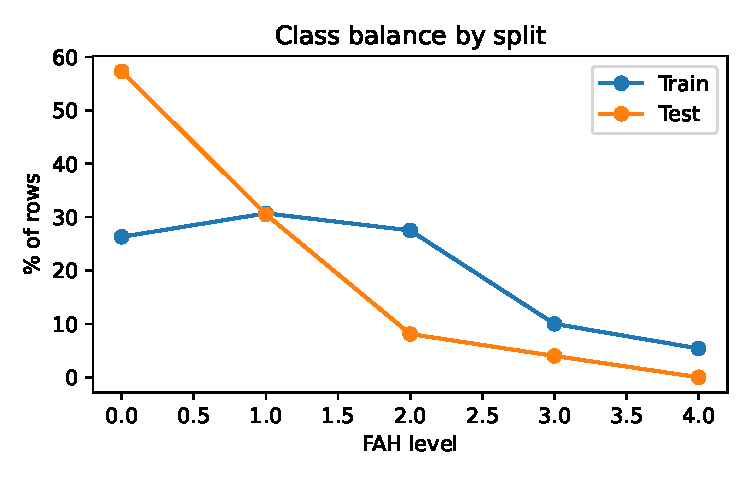
\includegraphics[keepaspectratio]{A1_Report_Full_Draft_files/figure-pdf/unnamed-chunk-36-1.pdf}}

}

\caption{Bar Plot illustrating FAH class balance by split.}

\end{figure}%

\subsubsection{Test Performance (Model vs
Baselines)}\label{test-performance-model-vs-baselines}

Below we compare the tuned LSTM-CORN model with three simple baselines.
We evaluate performance using four metrics: \textbf{Accuracy},
\textbf{Macro-F1}, \textbf{Mean Absolute Error (MAE)}, and
\textbf{Quadratic Weighted Kappa (QWK)}. Accuracy measures the
proportion of exact predictions but can be misleading under class
imbalance (e.g., always predicting the majority class). Macro-F1
computes precision and recall per class, takes their harmonic mean, and
averages equally across classes. This handles imbalance better but
ignores class ordering. MAE uses the ordinal scale directly, averaging
absolute differences between true and predicted levels (e.g., a miss of
\(0 \to 1\) counts as 1, while \(0 \to 4\) counts as 4), with a range
from \(0\) to \(K - 1\). QWK is a chance-corrected agreement measure
that penalises larger ordinal gaps using quadratic weights. It ranges
from 1 (perfect) to 0 (chance) and can be less than 0 (worse than
chance), making it well suited to ordinal targets and useful for
validation.

\begin{verbatim}
                      Model       acc   macroF1       MAE       QWK
0  LSTM–CORN (tuned $\tau$)  0.647700  0.295273  0.433381  0.390027
1         Majority (global)  0.305358  0.093571  0.735420  0.000000
2       Majority (per-area)  0.392603  0.200081  0.755334  0.089535
3      Persistence (y[t-1])  0.719298  0.455616  0.329066  0.658770
\end{verbatim}

On the held-out test window, the \textbf{persistence rule} (predict
today as yesterday within area) is the strongest comparator:\\
\$ \text{QWK} \approx 0.659 \$, \$ \text{Accuracy} \approx 0.719 \$, \$
\text{MAE} \approx 0.329 \$, \$ \text{Macro-F1} \approx 0.456\$ The
tuned LSTM--CORN improves markedly over the two m \$ajority heuristics
but does not reach persistence, with \$ \text{QWK} \approx 0.390 \$, \$
\text{Accuracy} \approx 0.648 \$, \$ \text{MAE} \approx 0.433 \$, and \$
\text{Macro-F1} \approx 0.295 \$.\\
The majority baselines are near chance in ordinal agreement (global \$
\text{QWK} \approx 0 \$; per-area \$ \text{QWK} \approx 0.09 \$),
confirming that always picking the common class is not competitive.

To read these numbers: \textbf{QWK} (Quadratic Weighted Kappa) is our
most appropriate headline metric because it respects ordering,
penalising large misses more than adjacent ones (higher is better).
\textbf{MAE} reports the average absolute distance between forecast and
truth on the 0--4 scale (lower is better). \textbf{Accuracy} is
exact-match rate and can look flattering under imbalance, while
\textbf{Macro-F1} balances precision and recall across classes by giving
each class equal weight.

The pattern suggests the test period is highly persistent and skewed
toward lower hazard---there are no ``High'' days---so copying yesterday
is often correct and unusually hard to beat. Although the neural model
learns meaningful ordinal structure (clear gains over majority rules),
it trails persistence on this particular window, likely due to strong
day-to-day autocorrelation and a distribution shift between train and
test.

Class-wise performance is therefore uneven, with under-prediction at the
upper levels and most errors occurring between adjacent
categories---which QWK appropriately down-weights. In practice,
persistence remains the operational benchmark in stable regimes, while
the LSTM--CORN is most promising for anticipating changes in hazard; we
examine this further via the confusion matrix and per-class summaries.

\begin{verbatim}
Text(0.5, 1.0, 'QWK by model')
Text(0, 0.5, 'QWK')
([0, 1, 2, 3], [Text(0, 0, 'LSTM–CORN (tuned $\tau$)'), Text(1, 0, 'Majority (global)'), Text(2, 0, 'Majority (per-area)'), Text(3, 0, 'Persistence (y[t-1])')])
\end{verbatim}

\begin{figure}[H]

{\centering \pandocbounded{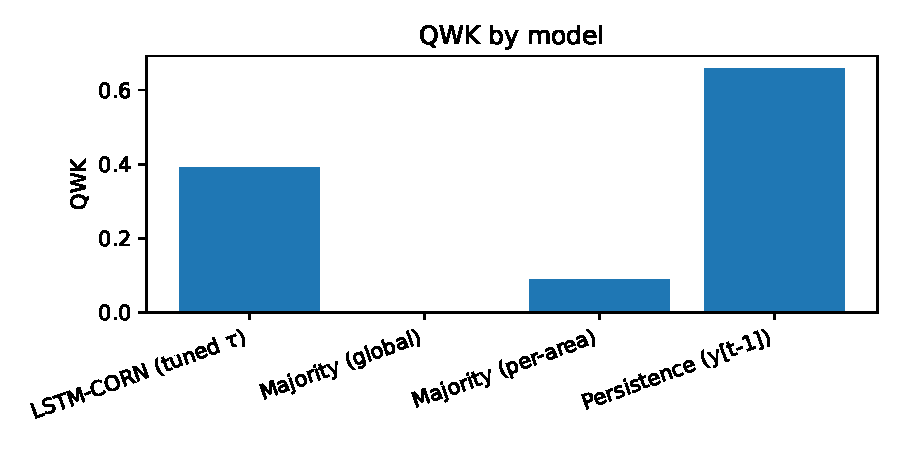
\includegraphics[keepaspectratio]{A1_Report_Full_Draft_files/figure-pdf/unnamed-chunk-38-3.pdf}}

}

\caption{Bar Chart depicting the QWK of the tuned LSTM-CORN model
compared to the three simple baselines.}

\end{figure}%

\subsubsection{Confusion Matrix and Per-Class
Report}\label{confusion-matrix-and-per-class-report}

The matrix shows a clear \textbf{ordinal pattern}. Class 0 is predicted
well (about \(0.90\) on the diagonal), with a small spill into class 1.
For class 1, only \(\sim 0.39\) stays on the diagonal, and \(\sim 0.58\)
is pushed down to 0; the model tends to \textbf{under-forecast} when
conditions are near the 0/1 boundary. Class 2 is mostly confused with
1ndefined (\(\approx 0.47\)) and sometimes with 0 (\(\approx 0.37\));
only \(\sim 0.16\) is correct. Class 3 is rarely predicted directly
(\(\sim 0.15\) diagonal) and is most often mapped to 1
(\(\approx 0.52\)) or 0 (\(\approx 0.31\)). There is effectively no
reliable signal for class 4 in the test window (support is 1 and it is
predicted as a 1), so per-class scores for 4 are unstable and shouldn't
be over-interpreted.

This pattern matches the aggregate metrics reported earlier: overall
accuracy and MAE are reasonable, but Macro-F1 and QWK suffer because the
model compresses higher hazards toward the centre/lower classes. In
other words, most errors are one-step, downward mistakes, good for
avoiding extreme over-calls but conservative relative to true highs.

If the operational goal is to catch more 2--3 days (accepting some extra
false alarms), you could lower the upper CORN thresholds slightly or use
a cost-sensitive tuning target. If the priority is minimising
over-warnings, the current calibration is aligned with that objective.

(array({[}0, 0, 0, \ldots, 0, 0, 0{]}), array({[}0, 0, 0, \ldots, 0, 0,
0{]}))

\begin{figure}[H]

{\centering \pandocbounded{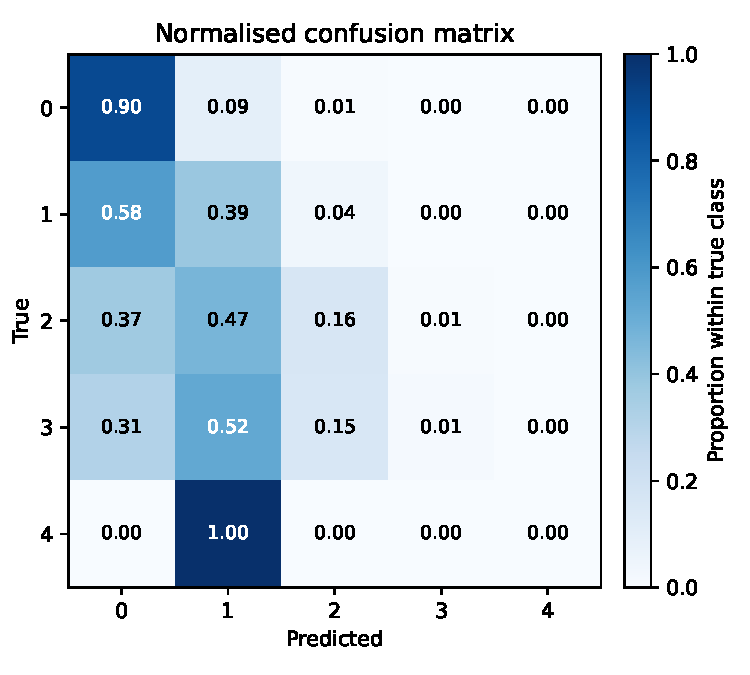
\includegraphics[keepaspectratio]{A1_Report_Full_Draft_files/figure-pdf/fig-cm-normalised-5.pdf}}

}

\caption{Normalised confusion matrix for the test set (rows sum to 1).
Numbers in cells are proportions.}

\end{figure}%

The matrix shows most mistakes are near-misses (adjacent categories),
which is consistent with the model optimising an ordinal metric.

\subsubsection{Effect of Threshold
Calibration}\label{effect-of-threshold-calibration}

Tuned monotone thresholds are intended to improve ordinal agreement over
the default \(0.5\) cut-offs.

\begin{verbatim}
        Cutoffs     acc   macroF1       MAE       QWK
0  tuned $\tau$  0.6477  0.295273  0.433381  0.390027
1      0.5 flat  0.6477  0.295273  0.433381  0.390027
\end{verbatim}

We re-evaluated the test set twice: once using the tuned monotone
thresholds \(\tau = [0.52, 0.50, 0.50, 0.48]\)\\
and once using flat \(0.5\) cut-offs for all CORN logits. The two runs
produced \textbf{identical} results:\\
Accuracy \(= 0.648\), Macro-F1 \(= 0.295\), MAE \(= 0.433\), QWK
\(= 0.390\).

This tells us that, on this test window, threshold calibration
\textbf{did not change any predicted labels}.\\
That is consistent with two facts: (i) the tuned \(\tau\) are very close
to \(0.5\), and (ii) most cumulative probabilities were far from the
decision boundaries, so nudging thresholds within \(0.48\)--\(0.52\)
doesn't flip classes.

This implies the model's test performance is driven by the sequence
model and learned representations, rather than by the post-hoc
thresholds. We keep the tuned \(\tau\) for completeness and because they
can help when class balance shifts, but we do \textbf{not} claim a
test-set gain from calibration here. If thresholding becomes more
influential (e.g., under stronger distribution shift), broader grids,
direct QWK optimisation, or area-specific \(\tau\) could be explored.

\subsubsection{Error Shape}\label{error-shape}

\begin{verbatim}
Mean abs error: 0.43338074917022285  | Median abs error: 0.0
\end{verbatim}

\begin{figure}[H]

{\centering \pandocbounded{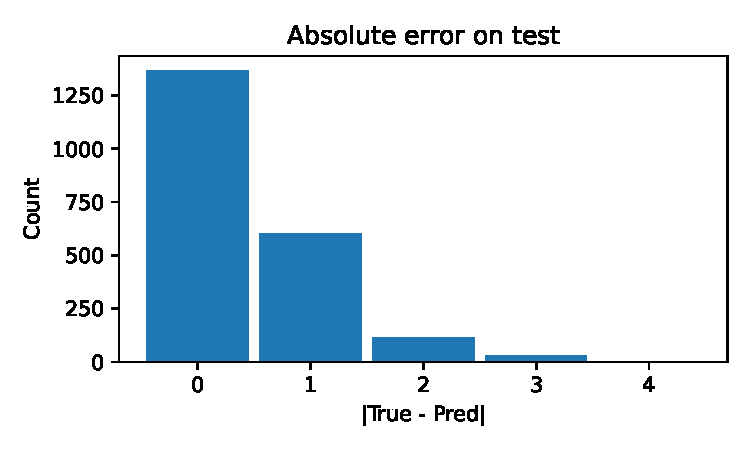
\includegraphics[keepaspectratio]{A1_Report_Full_Draft_files/figure-pdf/Error_shape-7.pdf}}

}

\caption{Histogram of absolute errors
\(|y_{    ext{true}} - y_{    ext{pred}}|\) on the test set. Bars are
centred at integer steps. Most errors are within one category,
consistent with MAE \(pprox 0.43\).}

\end{figure}%

The figure above shows the distribution of absolute errors
\(|y_{\text{true}} - y_{\text{pred}}|\) across FAH levels.\\
The model achieves an exact match on about 65\% of test days (error
\(= 0\)), and a further \(\sim 28\)--\(29\%\) are off by one category.
Only \(\sim 6\%\) are off by two and \(<1\%\) by three; no four-step
errors occur.

This aligns with the summary statistics (MAE \(\approx 0.43\), median
absolute error \(\approx 0\)):\\
in an ordinal setting, most misclassifications are near misses.
Operationally, this means the model is usually within one hazard step of
the issued level, even when it is wrong.

\subsection{Discussion}\label{discussion}

The held-out results paint a clear picture. Hazards in this period are
highly persistent and skewed toward the lower levels, and the naive
persistence rule (``predict today as yesterday within area'') performs
very strongly on all summary metrics. Our tuned LSTM--CORN improves
markedly over the two majority baselines, but it does not beat
persistence on this particular test window.

\subsubsection{Metrics \& Diagnostics}\label{metrics-diagnostics}

Accuracy and MAE are reasonable for the neural model, but the QWK and
macro-F1 show performance drops higher up the scale. This is consistent
with the near-diagonal confusion matrix that has a downward bias (Level
1 is often pushed to 0; Levels 2--3 are frequently mapped to 1) while
extreme over-calls are rare. The error histogram shows most misses are
within one category (consistent with MAE \(\approx 0.43\)): useful for
avoiding false alarms, but conservative relative to true highs. Finally,
threshold calibration had almost no effect (tuned
\(\tau \approx [0.52, 0.50, 0.50, 0.48]\) and gave identical results to
0.5), which implies the limiting factor is representation/sequence
learning, not the label cut-offs.

\subsubsection{Why persistence wins
here}\label{why-persistence-wins-here}

Two data realities favour the \(y[t-1]\) rule:\\
(i) \textbf{strong day-to-day autocorrelation} in FAH;\\
(ii) \textbf{imbalance and shift:} the test window contains no ``High''
days and is dominated by Levels 0--1. In that regime, copying yesterday
is genuinely hard to beat. The LSTM--CORN learns the ordinal structure
and avoids wild swings, but with few upper-level examples and a short
14-day context, it struggles to escalate to 2--3 when the series does
move.

\subsubsection{Operational
interpretation}\label{operational-interpretation}

If the near-term goal is to minimise false alarms, the current
calibration is acceptable: errors are mostly one-step and downward. If
instead the priority is to catch emerging higher hazards, you would
tolerate more false positives and lower the effective thresholds for the
top levels (a cost-sensitive calibration). Either way, persistence
remains a strong benchmark, and the neural-persistence disagreements are
useful review flags.

\subsubsection{Limitations}\label{limitations}

Conclusions are conditioned on this split: the test window lacks class 4
entirely and has very few class 3 days, so per-class scores at the top
end are unstable. The dataset is modest for sequence models, labels may
contain operational noise, and we restricted the model to observed
histories (no external forecasts), which caps lead-time sensitivity. We
mitigated leakage with forward-chaining folds and an embargo, but
results will vary with split point and winter severity.

\subsubsection{Possible Future
Improvements}\label{possible-future-improvements}

Short-to-medium steps that fit the current pipeline: - \textbf{Longer
and/or multi-scale context} (e.g., 28--45 days plus recent 7-day summary
features) to help detect trend changes.\\
- \textbf{Area- or season-specific calibration} of \(\tau\), or a simple
\textbf{cost-sensitive threshold} that weights upward errors more
heavily.\\
- \textbf{Richer dynamics}: include forecasted weather (when available)
and simple change features (day-to-day deltas, 7-day slopes).\\
- \textbf{Ordinal-aware loss variants} (e.g., ordinal focal/Tversky) to
emphasise rare upward moves without exploding false alarms.\\
- \textbf{Modeling with persistence} rather than against it: feed
\(y[t-1]\) explicitly (we already include it) and/or ensemble the neural
model with the persistence rule; use the ensemble to trigger escalation
only when both agree.

For this winter slice, FAH rewards yesterday-equals-today. The
LSTM--CORN gives mostly one-step, conservative predictions and clearly
outperforms majority rules, but not persistence. With more
imbalance-aware training, longer context, and cost-sensitive calibration
or ensembling, it should provide earlier and more reliable hazard
signals while retaining low false-alarm rates.

\subsection{Conclusion}\label{conclusion}

This work developed a reproducible pipeline for ordinal avalanche
forecasting, combining structured data preparation, time-aware
validation, and an LSTM--CORN model adjusted for class imbalance and
monotone decision thresholds. On the held-out test window, the neural
model outperforms both majority baselines but does not surpass
persistence. This is expected given the strong day-to-day
autocorrelation and the concentration of FAH at lower levels during this
period.

The diagnostics are consistent with this outcome. The confusion matrix
is near-diagonal with a slight downward bias, MAE (\(\approx 0.43\))
indicates that most errors fall within one category, and threshold
calibration has negligible effect. This suggests that the main
limitations lie in the data regime and sequence representation rather
than in the choice of decision cut-offs.

From an operational perspective, the model is conservative and unlikely
to produce extreme over-warnings. Its greatest value is in cases where
it diverges from persistence, indicating potential changes in hazard.
Sensitivity to rising risk could be improved through longer or
multi-scale look-back periods, cost-sensitive or area- and
season-specific calibration, the inclusion of forecasted weather and
change features, and the use of ordinal focal or Tversky losses, or
ensembling with persistence.

Additional ``High'' days and further winters will help stabilise
estimates at the upper levels. Overall, the method is interpretable and
extensible. With targeted refinements, it has the potential to provide
earlier and more reliable indicators of increasing avalanche hazard
while maintaining a low false alarm rate.

\subsection{References}\label{references}

\begin{itemize}
\item
  Statham, G., Haegeli, P., Greene, E., Birkeland, K., Israelson, C.,
  Tremper, B. and Kelly, J. (2018) `A conceptual model of avalanche
  hazard', \emph{Natural Hazards}, 90(2), pp.~663--691.
  \url{https://doi.org/10.1007/s11069-017-3070-5}.
\item
  Cui, Y., Jia, M., Lin, T.-Y. and Song, Y. (2019) `Class-Balanced Loss
  Based on Effective Number of Samples', in \emph{Proceedings of the
  IEEE/CVF Conference on Computer Vision and Pattern Recognition
  (CVPR)}, pp.~9268--9277.
  \url{https://doi.org/10.1109/CVPR.2019.00949}.
\item
  Shi, X., Cao, W. and Raschka, S. (2021) `Deep Neural Networks for
  Rank-Consistent Ordinal Regression Based on Conditional
  Probabilities', \emph{arXiv preprint} arXiv:2111.08851. Available at:
  \url{https://arxiv.org/abs/2111.08851}.
\item
  Lim, B. and Zohren, S. (2021) `Time-series forecasting with deep
  learning: a survey', \emph{Philosophical Transactions of the Royal
  Society A: Mathematical, Physical and Engineering Sciences},
  379(2194), 20200209. \url{https://doi.org/10.1098/rsta.2020.0209}.
\end{itemize}

\subsection{Appendix}\label{appendix}

\subsubsection{Data Figures}\label{data-figures}

After consolidation, \(99.9\%\) of (\texttt{Date}, \texttt{OSgrid},
\texttt{Area}) keys were unique.\\
We found \(12\) keys with duplicates (\(8\) keys with 2 rows; \(4\) with
\(\geq 3\)).\\
Conflict cases were retained and flagged; duplicates that differed only
by missingness were collapsed (4 rows collapsed).

\subsubsection{Model / Results Figures}\label{model-results-figures}

\begin{verbatim}
<matplotlib.colorbar.Colorbar object at 0x00000286E4ACFDD0>
\end{verbatim}

\begin{figure}[H]

{\centering \pandocbounded{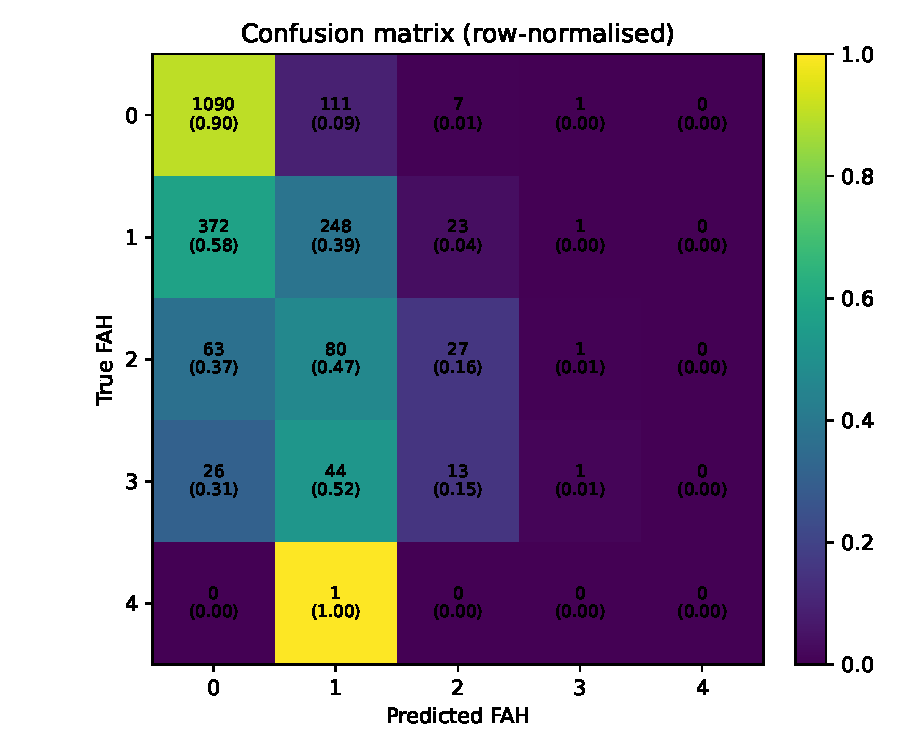
\includegraphics[keepaspectratio]{A1_Report_Full_Draft_files/figure-pdf/unnamed-chunk-50-1.pdf}}

}

\caption{Figure B1: Confusion matrix on the test set; numbers show
counts (top) and row-normalised rates (bottom)}

\end{figure}%

\begin{verbatim}
<BarContainer object of 5 artists>
\end{verbatim}

\begin{verbatim}
<BarContainer object of 5 artists>
\end{verbatim}

\begin{verbatim}
<BarContainer object of 5 artists>
\end{verbatim}

\begin{verbatim}
[<matplotlib.axis.XTick object at 0x00000286E4B45E90>, <matplotlib.axis.XTick object at 0x00000286E4B4D150>, <matplotlib.axis.XTick object at 0x00000286E4A66810>, <matplotlib.axis.XTick object at 0x00000286E4BB8290>, <matplotlib.axis.XTick object at 0x00000286E4BBA4D0>]
[Text(0, 0, '0'), Text(1, 0, '1'), Text(2, 0, '2'), Text(3, 0, '3'), Text(4, 0, '4')]
\end{verbatim}

\begin{verbatim}
(0.0, 1.05)
\end{verbatim}

\begin{verbatim}
Text(0.5, 0, 'FAH level')
Text(0, 0.5, 'Score')
\end{verbatim}

\begin{verbatim}
Text(0.5, 1.0, 'Per-class precision/recall/F1 (test)')
\end{verbatim}

\begin{verbatim}
<matplotlib.legend.Legend object at 0x00000286E4878C10>
\end{verbatim}

\begin{figure}[H]

{\centering \pandocbounded{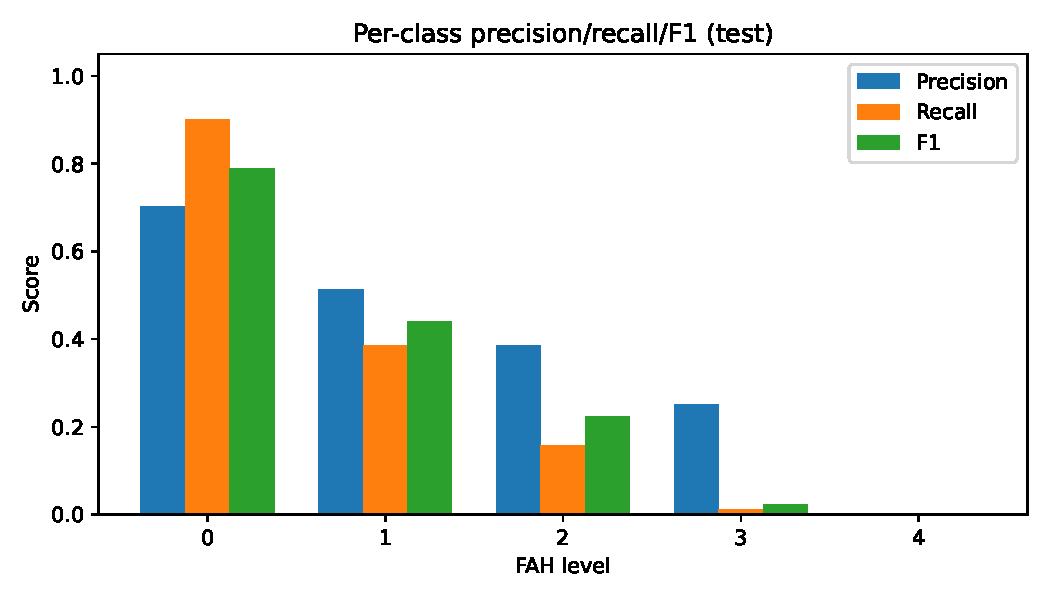
\includegraphics[keepaspectratio]{A1_Report_Full_Draft_files/figure-pdf/unnamed-chunk-51-3.pdf}}

}

\caption{Figure B2: Per-class precision, recall, and F1 on the test
set.}

\end{figure}%

\begin{verbatim}
<BarContainer object of 4 artists>
\end{verbatim}

\begin{verbatim}
Text(0.5, 1.0, 'Quadratic Weighted Kappa')
\end{verbatim}

\begin{verbatim}
(-0.1, 0.7587704965742034)
\end{verbatim}

\begin{verbatim}
<BarContainer object of 4 artists>
\end{verbatim}

\begin{verbatim}
Text(0.5, 1.0, 'Mean Absolute Error')
\end{verbatim}

\begin{verbatim}
Text(0.5, 0.98, 'Model vs. baselines on test')
\end{verbatim}

\begin{figure}[H]

{\centering \pandocbounded{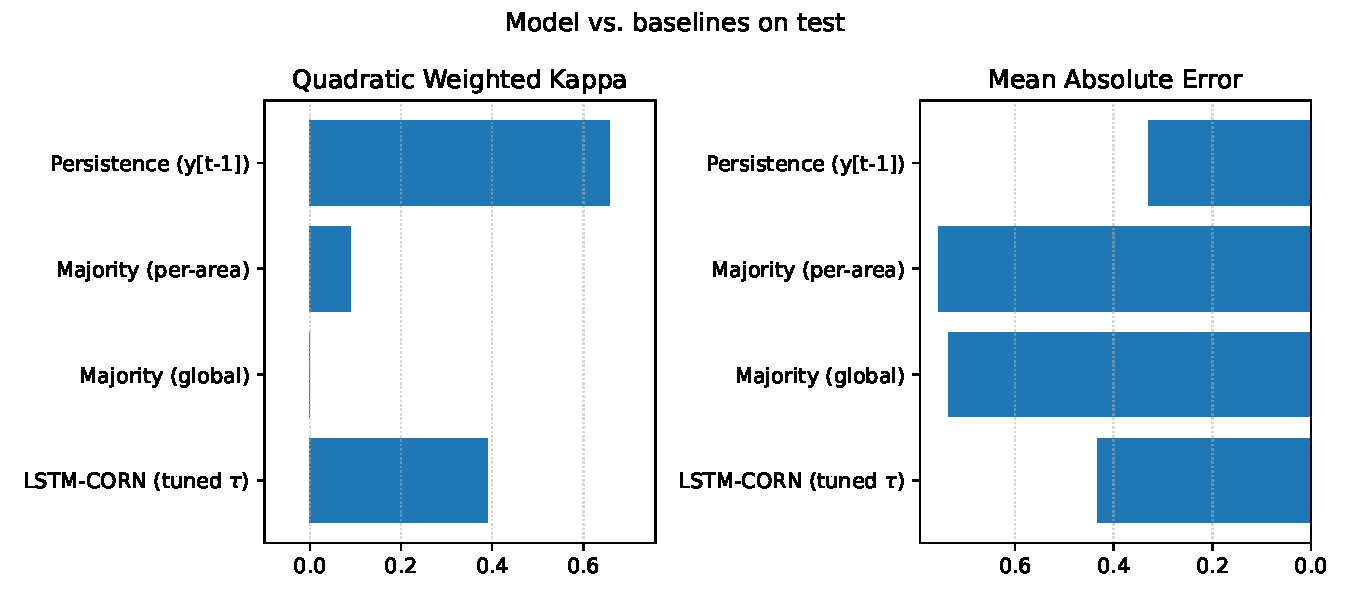
\includegraphics[keepaspectratio]{A1_Report_Full_Draft_files/figure-pdf/unnamed-chunk-52-5.pdf}}

}

\caption{Figure B3: Comparison of the neural model to baselines on QWK
(higher is better) and MAE (lower is better).}

\end{figure}%

\begin{verbatim}
<BarContainer object of 4 artists>
\end{verbatim}

\begin{verbatim}
Text(1, 0.5199999809265137, '0.50')
Text(2, 0.5199999809265137, '0.50')
Text(3, 0.5199999809265137, '0.50')
Text(4, 0.4000000059604645, '0.38')
\end{verbatim}

\begin{verbatim}
[<matplotlib.axis.XTick object at 0x00000286E4CC2D10>, <matplotlib.axis.XTick object at 0x00000286DD5D3BD0>, <matplotlib.axis.XTick object at 0x00000286E4CB3FD0>, <matplotlib.axis.XTick object at 0x00000286E4D1AE10>]
[Text(1, 0, '$\\tau$1'), Text(2, 0, '$\\tau$2'), Text(3, 0, '$\\tau$3'), Text(4, 0, '$\\tau$4')]
\end{verbatim}

\begin{verbatim}
(0.0, 1.05)
\end{verbatim}

\begin{verbatim}
Text(0, 0.5, 'Threshold value')
\end{verbatim}

\begin{verbatim}
Text(0.5, 1.0, 'Tuned CORN thresholds (monotone)')
\end{verbatim}

\begin{figure}[H]

{\centering \pandocbounded{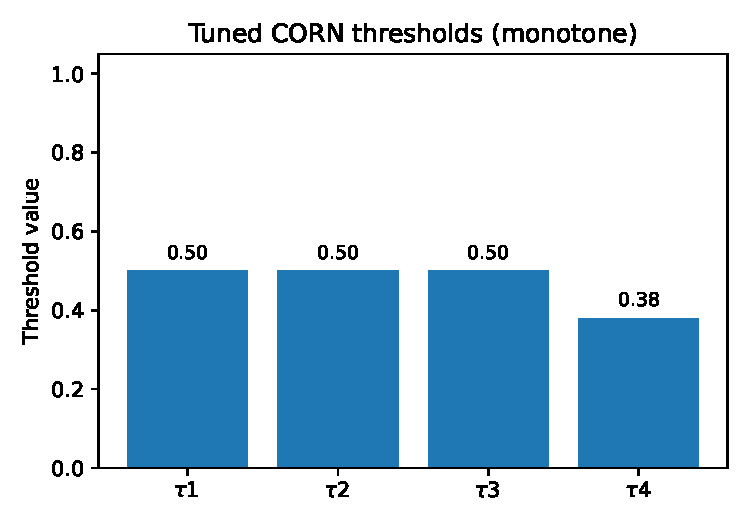
\includegraphics[keepaspectratio]{A1_Report_Full_Draft_files/figure-pdf/unnamed-chunk-53-7.pdf}}

}

\caption{Figure B4: Tuned CORN decision thresholds (\(\tau\)) used to
convert probabilities into ordinal labels.}

\end{figure}%

\begin{verbatim}
<BarContainer object of 5 artists>
\end{verbatim}

\begin{verbatim}
<BarContainer object of 5 artists>
\end{verbatim}

\begin{verbatim}
[<matplotlib.axis.XTick object at 0x00000286E4AD9C10>, <matplotlib.axis.XTick object at 0x00000286E4D78690>, <matplotlib.axis.XTick object at 0x00000286E4D42D10>, <matplotlib.axis.XTick object at 0x00000286E4D56310>, <matplotlib.axis.XTick object at 0x00000286E4D24610>]
[Text(0, 0, '0'), Text(1, 0, '1'), Text(2, 0, '2'), Text(3, 0, '3'), Text(4, 0, '4')]
\end{verbatim}

\begin{verbatim}
(0.0, 1.05)
\end{verbatim}

\begin{verbatim}
Text(0.5, 0, 'FAH level')
Text(0, 0.5, 'Proportion')
\end{verbatim}

\begin{verbatim}
Text(0.5, 1.0, 'Class balance by split (window targets)')
\end{verbatim}

\begin{verbatim}
<matplotlib.legend.Legend object at 0x00000286E4C613D0>
\end{verbatim}

\begin{figure}[H]

{\centering \pandocbounded{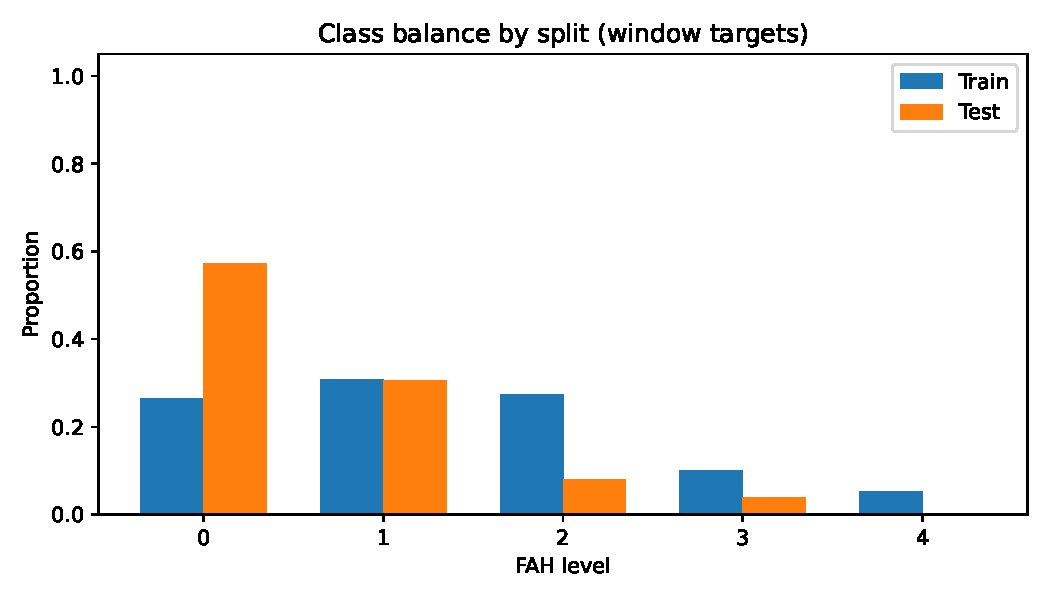
\includegraphics[keepaspectratio]{A1_Report_Full_Draft_files/figure-pdf/unnamed-chunk-54-9.pdf}}

}

\caption{Figure B5: Proportion of FAH levels at the window level (what
the LSTM actually trained on) in train vs test.}

\end{figure}%




\end{document}
